%Marco
\section{Design}
Um den Spielern des Planspiels auch ein echtes Spielerlebnis zu bieten wurde die
Entscheidung getroffen eine grafische Oberfl�che zu schaffen, welche jegliche Spielinformationen abbildet. 
Auf den folgenden Seiten wird der Entwicklungsprozess, als auch die Ergebnisse
und m�gliche Verbesserungsm�glichkeiten wiedergegeben:

\subsection{Entwicklung} 
Die Entwicklung des Designs spielte eine wichtige Rolle bei uns, welche sich in einzelne Phasen unterteilen lassen kann. 
Die einzelnen Phasen, Schritte und Ideen dahinter werden im folgenden dargelegt.

\subsubsection{Brainstorming \& erste Skizzen}
Nach der Entwicklung des Spielkonzeptes und der Programmierung der ersten
Spielfunktionen wurde damit begonnen die ersten Ideen f�r das User-Interface zu sammeln. 
Dazu wurde eine gemeinsame Brainstorming-Session gestartet und alle m�glichen
Vorschl�ge zusammengetragen. Diese Vorschl�ge wurden dann in erste Skizzen
verpackt und m�gliche Anordnungen und Elemente diskutiert. 
Da die Skizzen jedoch sehr einfach, un�bersichtlich \& ungenau waren wurden
daraus, mit Hilfe von Grafikprogramme, Mockups erstellt, um die Ideen
realit�tsgenau darzustellen und  wirken zu lassen und somit sowohl St�rken als
auch Schw�chen der Ideen aufzudecken.

\begin{figure}[H]
\centering
\centering
\includegraphics[width=0.8\textwidth]{se-wa-jpg/gui_skizze}
\caption{Eine der ersten Skizzen aus dem Brainstorming}
\label{Eine der ersten Skizzen aus dem Brainstorming}
\end{figure}

\subsubsection{Mockup \& Ideen}
Im folgenden werden die einzelnen Mockup-Grafiken dargestellt und kurz
erl�utert:

\paragraph{Elemente}
Um den Spieler nicht zu verwirren wird auf statische Oberfl�chenelemente
gesetzt, welche sich in jedem Bildschirm an der selben Stellen befinden. Daf�r
wurde der Bildschirm der Mockups in drei Teile geteilt:
\begin{itemize}
\item Men�leiste
\item Hauptframe
\item Sidebar
\end{itemize}

Die \textbf{Men�leiste} befindet sich am oberen Bildschirmrand und stellt dem
Spieler die Navigation auf die unterschiedlichen Seiten zur Verf�gung.

Im \textbf{Hauptfrage} werden die Hauptinformationen des Spiels dargestellt und
ist f�r die Hauptinteraktionen verantwortlich.

Die \textbf{Sidebar} dient dabei als Erweiterung und bietet zus�tzliche
Informationen, aber auch Interaktionsm�glichkeiten an.

\paragraph{Unternehmens�bersicht}
Die Idee hinter der Unternehmens�bersicht ist, dass der Spieler einen �berblick
�ber alle wichtigen Informationen seines Unternehmens bekommt. Dazu z�hlt der
Kontostand, Einnahmen, Ausgaben, Anzahl der Rohstoffe, Stromproduktion,
Stromverbrauch, Strombilanz und die Anzahl der im Besitz befindenen Kraftwerke & Mienen. Des Weiteren soll der Nutzer auf dieser Seite auch �ber Aktionen der vorangegangen Spielrunde informiert werden, um keine wichtigen Interkationen & Ereignisse zu verpassen.
\begin{figure}[H]
\centering
\centering
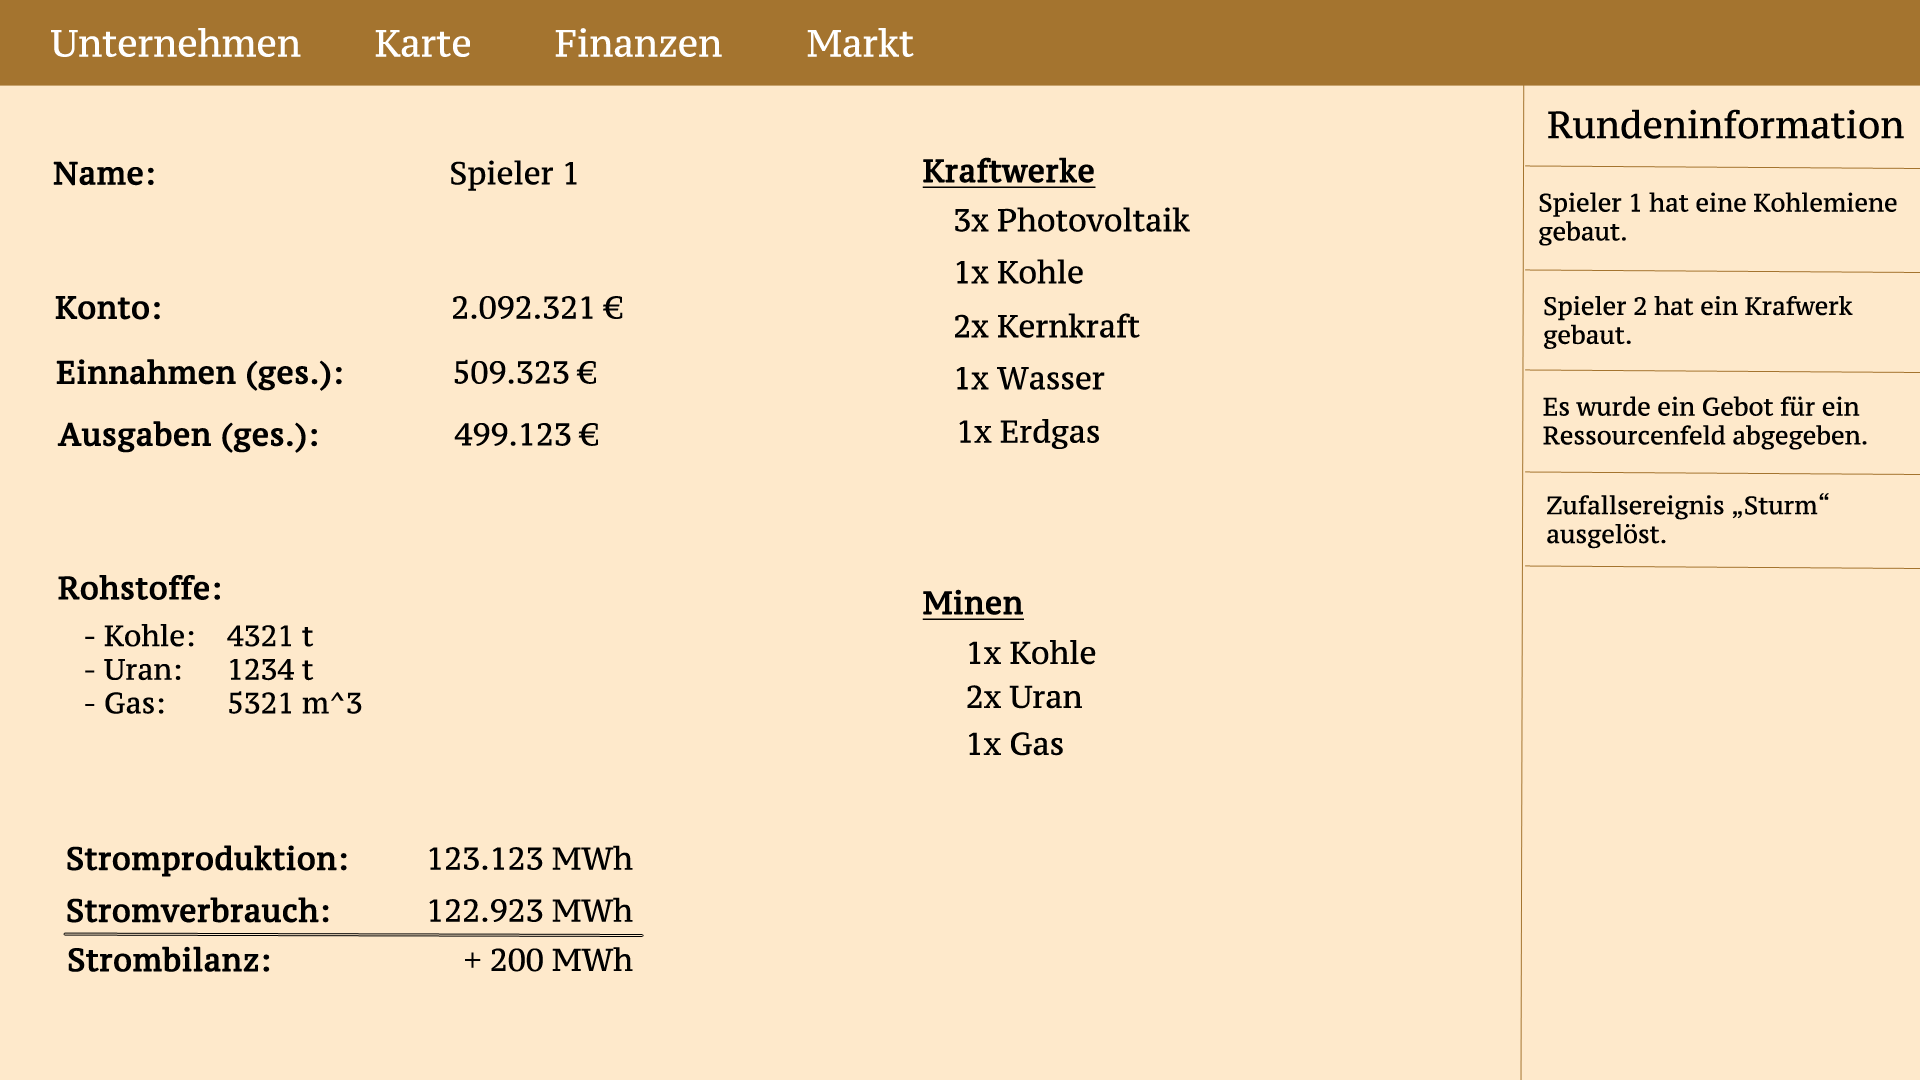
\includegraphics[width=0.9\textwidth]{se-wa-jpg/gui_unternehmen}
\caption{Unternehmens�bersicht}
\label{Unternehmens�bersicht}
\end{figure}

\paragraph{Karte mit ausgew�hltem Ressourcenfeld}
\begin{figure}[H]
\centering
\centering
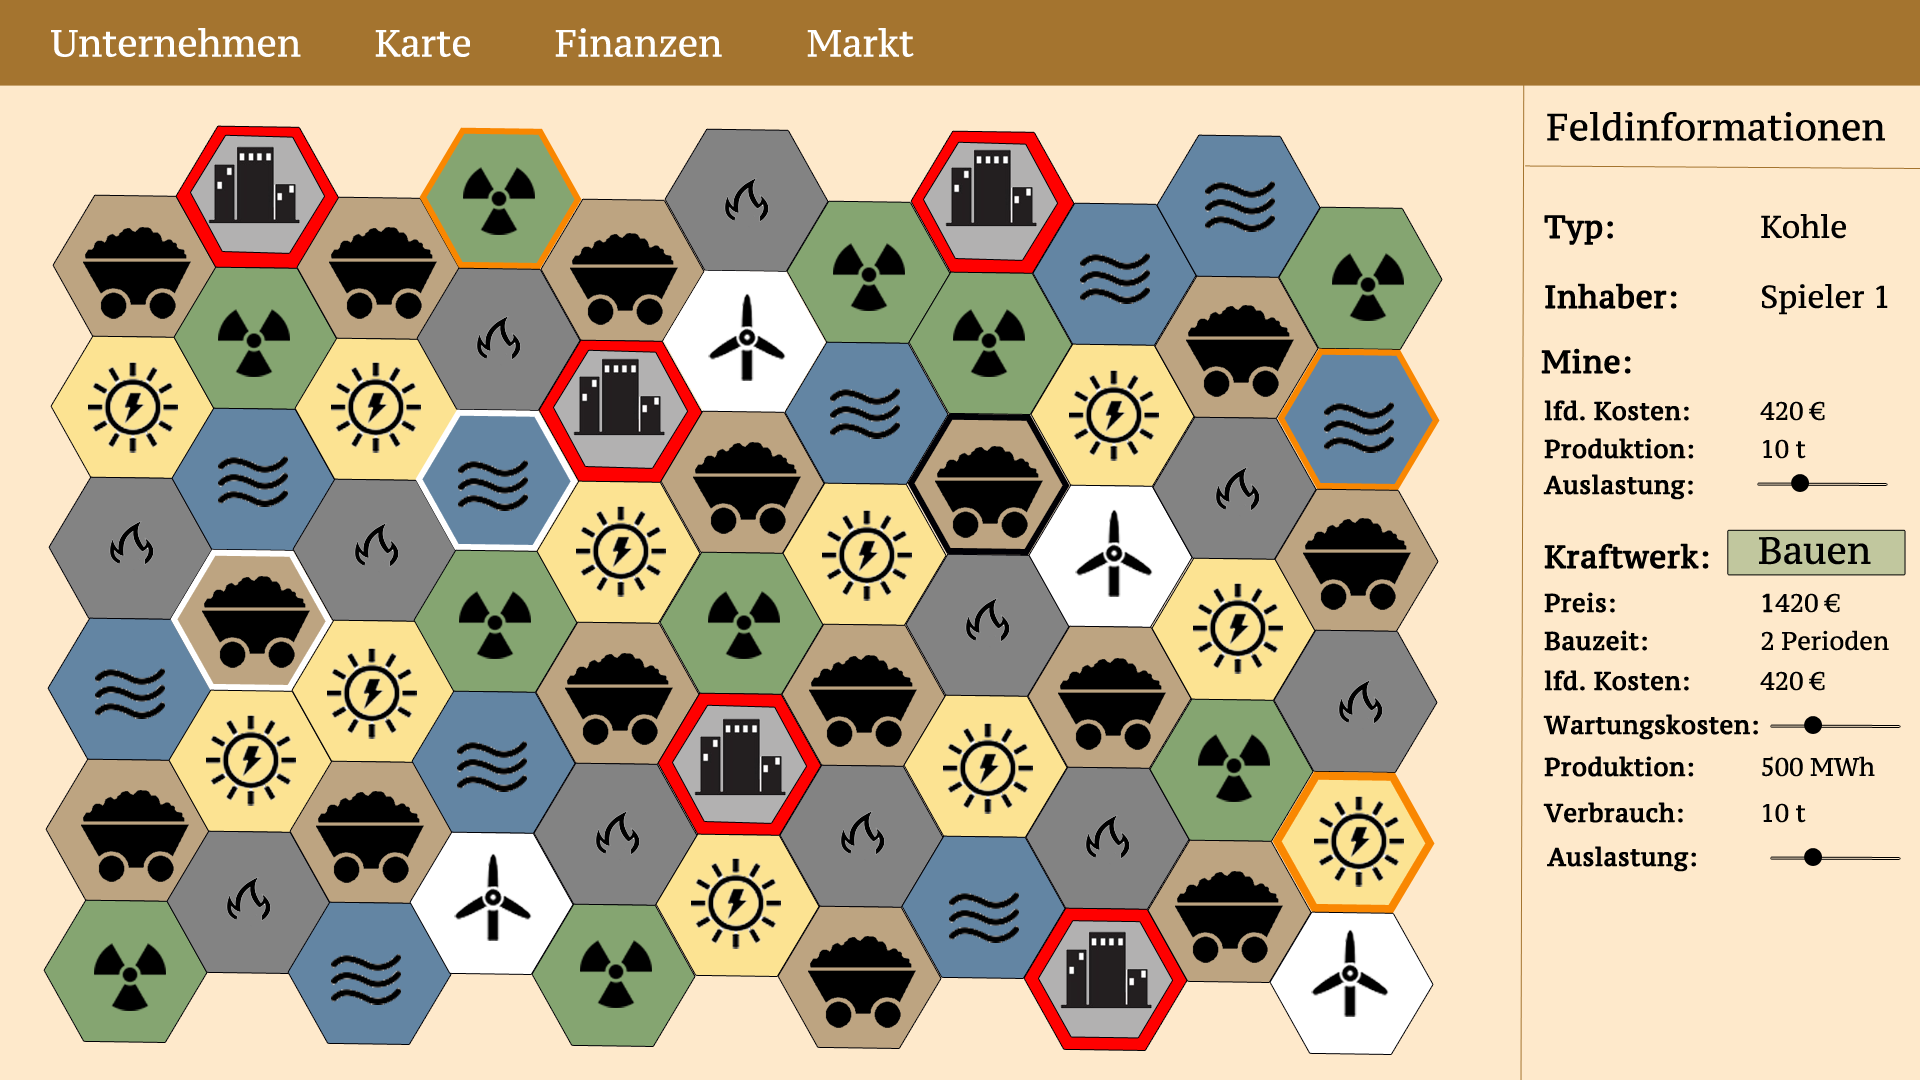
\includegraphics[width=0.9\textwidth]{se-wa-jpg/gui_karte01}
\caption{Karte mit ausgew�hltem Ressourcenfeld}
\label{Karte mit ausgew�hltem Ressourcenfeld}
\end{figure}

\paragraph{Karte mit ausgew�hlter Stadt}
\begin{figure}[H]
\centering
\centering
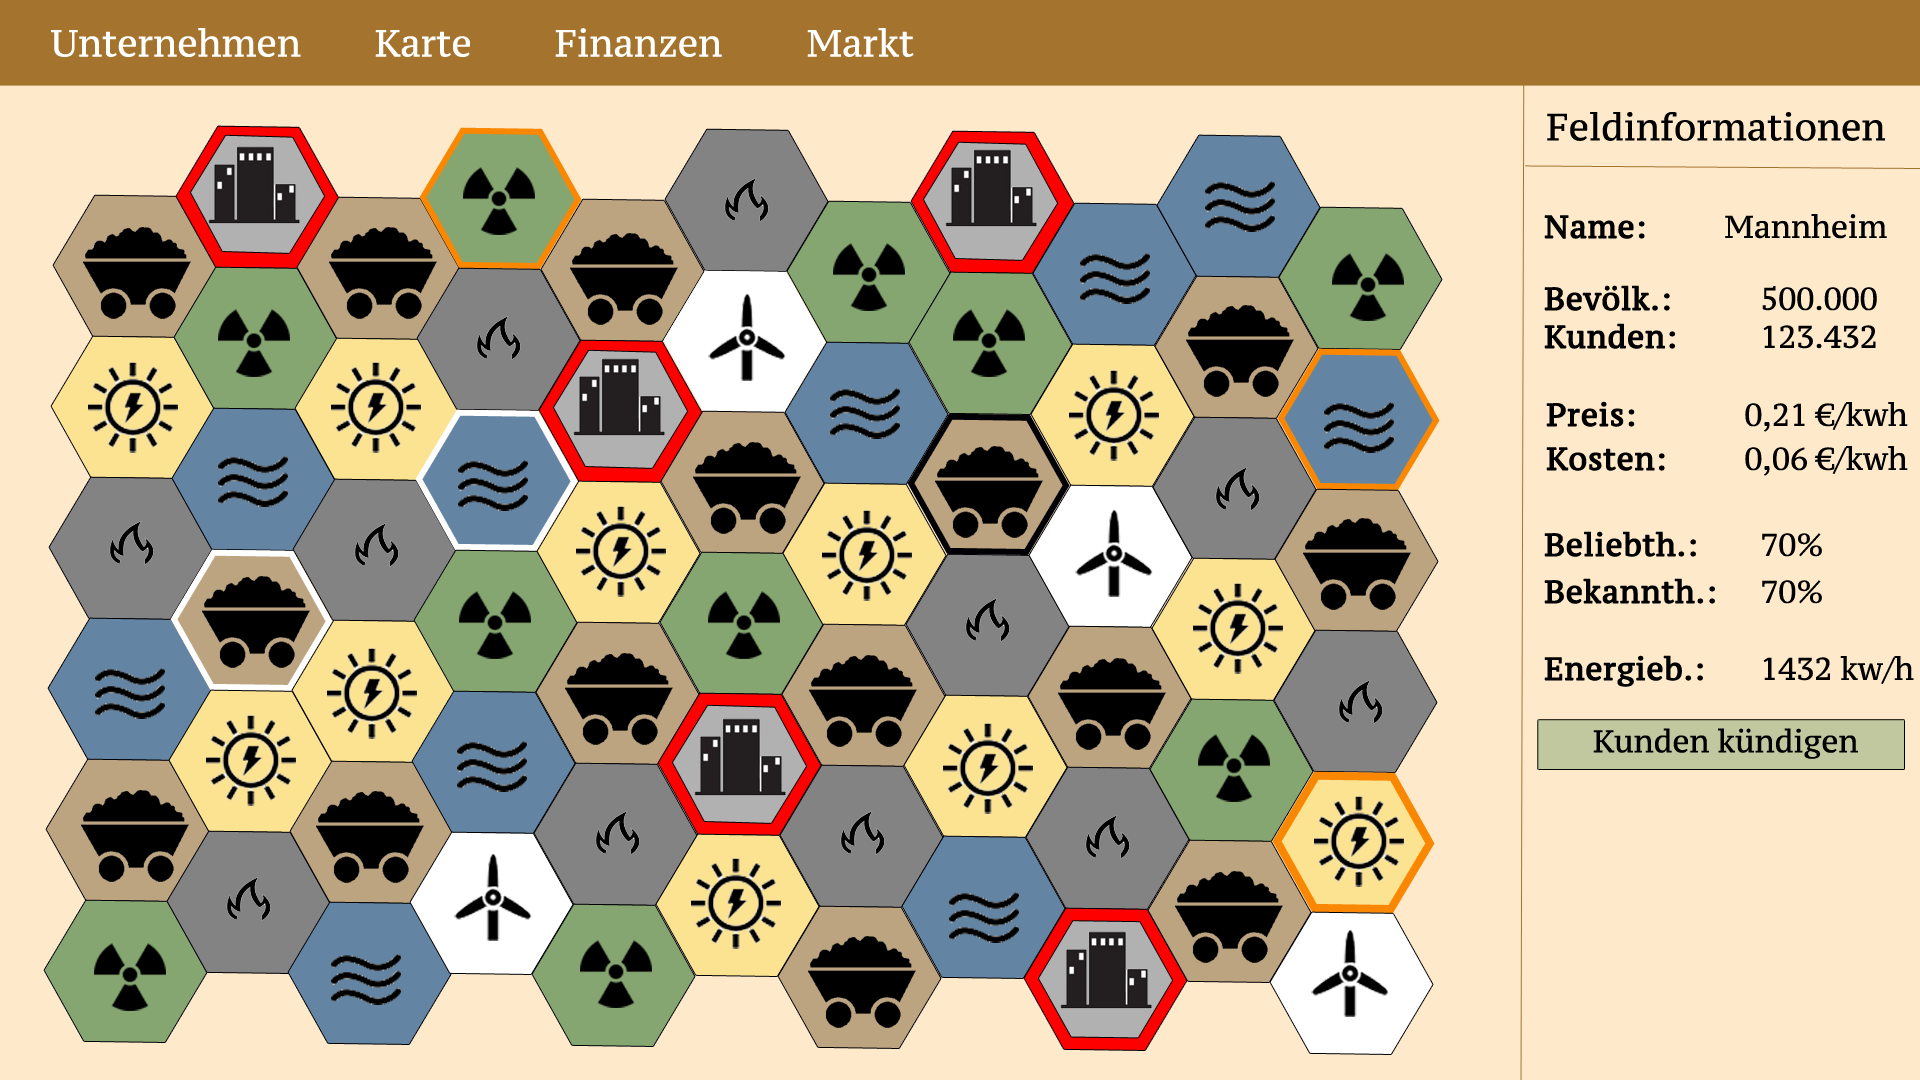
\includegraphics[width=0.9\textwidth]{se-wa-jpg/gui_karte02}
\caption{Karte mit ausgew�hlter Stadt}
\label{Karte mit ausgew�hlter Stadt}
\end{figure}

\paragraph{Finanzen}
\begin{figure}[H]
\centering
\centering
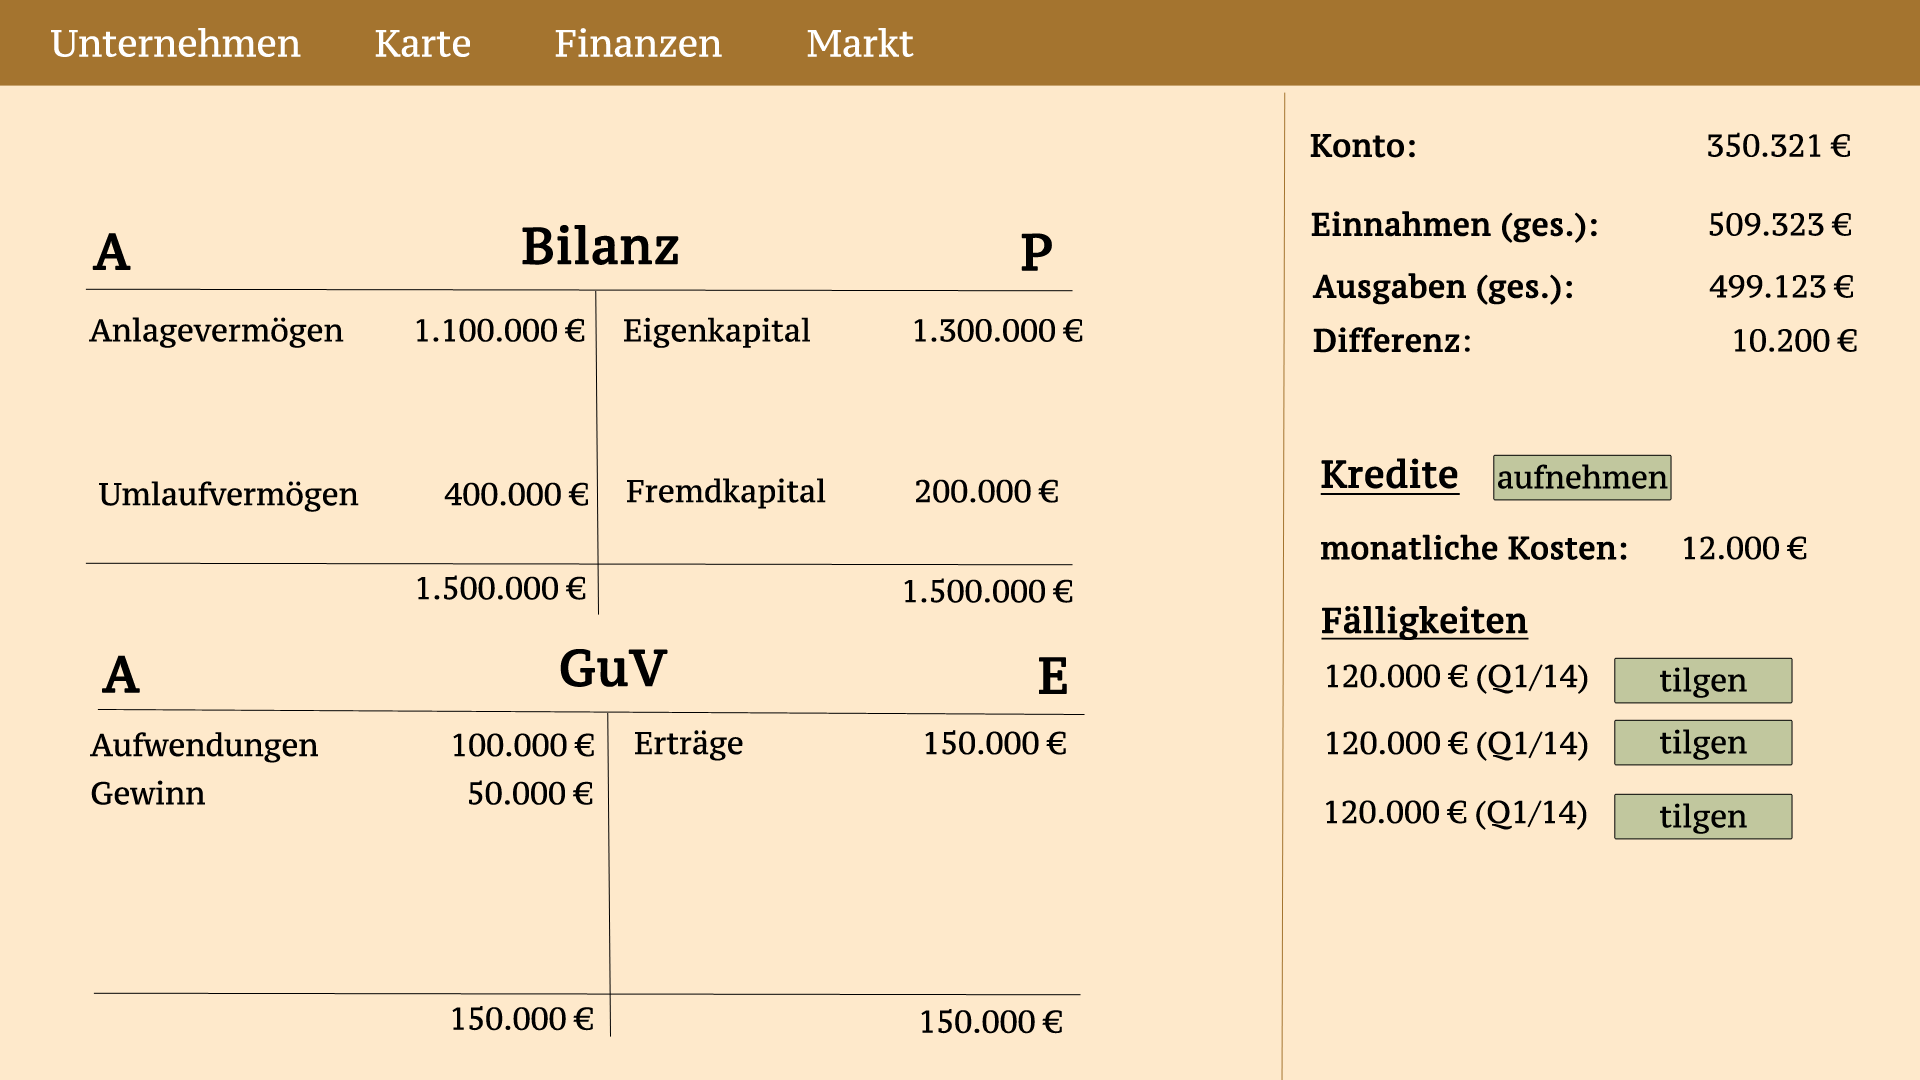
\includegraphics[width=0.9\textwidth]{se-wa-jpg/gui_finanzen}
\caption{Finanzen}
\label{Finanzen}
\end{figure}

\paragraph{Markt}
\begin{figure}[H]
\centering
\centering
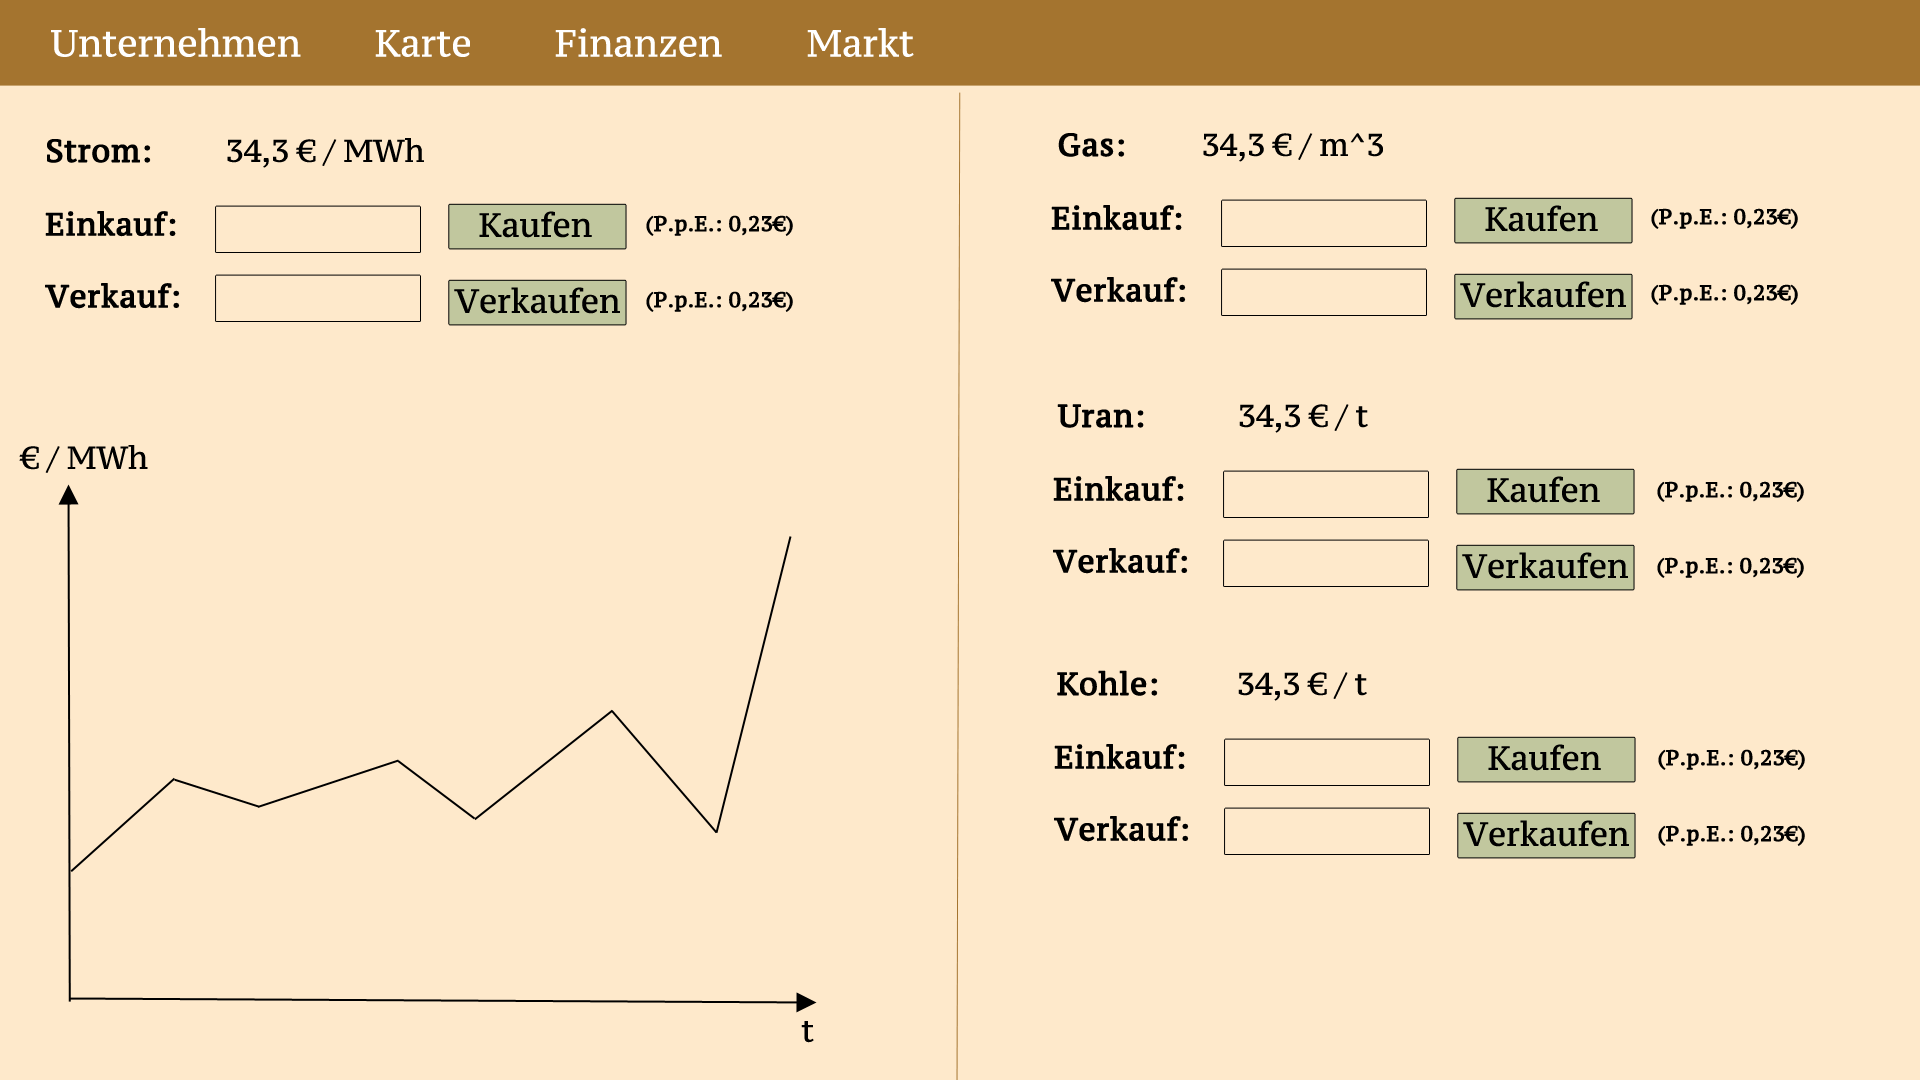
\includegraphics[width=0.9\textwidth]{se-wa-jpg/gui_markt}
\caption{Markt}
\label{Markt}
\end{figure}

\subsection{Auswertung}
\subsubsection{Ergebnis}

\subsubsection{Vergleich Mockup mit Ergebnis}
\subsubsection{Verbesserungsm�glichkeiten}